\documentclass[letterpaper,12pt,fleqn]{article}
\usepackage{matharticle}
\usepackage{tikz}
\usepackage{array}
\pagestyle{empty}
\newcommand{\T}{\mathscr{T}}
\newcommand{\U}{\mathcal{U}}
\newcommand{\e}{\epsilon}
\renewcommand{\d}{\delta}
\renewcommand{\a}{\alpha}
\renewcommand{\l}{\lambda}
\renewcommand{\C}{\checkmark}
\newcommand{\X}{\(\bigtimes\)}
\newcommand{\A}{
  \begin{minipage}{1in}
    \(X\) finite: \C \\
    \(X\) infinite: \X
  \end{minipage}
}
\newcommand{\B}{
  \begin{minipage}{1.5in}
    \(X\) countable: \C \\
    \(X\) uncountable: \X
  \end{minipage}
}
\begin{document}
\section*{Separation}

\begin{definition}[\(T_1\)]
  Let \(X\) be a topological space.  To say that \(X\) is a \(T_1\)\emph{-space} means that for all distinct
  \(x,y\in X\) there exists \(U,V\in\T\) such that \(x\in U\), \(y\notin U\) and \(x\notin V\), \(y\in V\).
  \begin{center}
    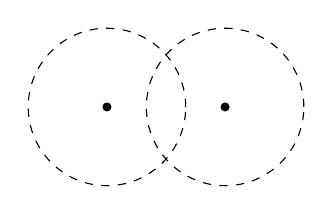
\begin{tikzpicture}
      \draw [dashed] (0,0) circle [radius=1];
      \draw [dashed] (1.5,0) circle [radius=1];
      \draw [fill] (0,0) circle [radius=0.05];
      \draw [fill] (1.5,0) circle [radius=0.05];
    \end{tikzpicture}
  \end{center}
\end{definition}

\begin{definition}[\(T_2\)]
  Let \(X\) be a topological space.  To say that \(X\) is \(T_2\)\emph{-space} or \emph{Hausdorff} means that for
  all distinct \(x,y\in X\) there exists disjoint \(U,V\in\T\) such that \(x\in U\) and \(y\in V\).
  \begin{center}
    \begin{tikzpicture}
      \draw [dashed] (0,0) circle [radius=1];
      \draw [dashed] (2.25,0) circle [radius=1];
      \draw [fill] (0,0) circle [radius=0.05];
      \draw [fill] (2.25,0) circle [radius=0.05];
    \end{tikzpicture}
  \end{center}
\end{definition}

\begin{definition}[Regular]
  Let \(X\) be a topological space.  To say that \(X\) is \emph{regular} means that for all \(x\in X\) and closed
  sets \(A\subset X\) such that \(x\notin A\) there exists disjoint \(U,V\in\T\) such that \(x\in U\) and
  \(A\subset V\).
  \begin{center}
    \begin{tikzpicture}
      \draw [dashed] (0,0) circle [radius=1];
      \draw [dashed] (2.25,0) circle [radius=1];
      \draw [fill] (0,0) circle [radius=0.05];
      \draw (2,-0.2) rectangle (2.5,0.2);
    \end{tikzpicture}
  \end{center}
  To say that \(X\) is a \(T_3\)\emph{-space} means that \(X\) is regular and \(T_1\).
\end{definition}

\begin{definition}[Normal]
  Let \(X\) be a topological space.  To say that \(X\) is \emph{regular} means that for all disjoint closed sets
  \(A,B\subset X\) there exists disjoint \(U,V\in\T\) such that \(A\subset U\) and \(B\subset V\).
  \begin{center}
    \begin{tikzpicture}
      \draw [dashed] (0,0) circle [radius=1];
      \draw [dashed] (2.25,0) circle [radius=1];
      \draw (-0.25,-0.2) rectangle (0.25,0.2);
      \draw (2,-0.2) rectangle (2.5,0.2);
    \end{tikzpicture}
  \end{center}
  To say that \(X\) is a \(T_4\)\emph{-space} means that \(X\) is normal and \(T_1\).
\end{definition}

\begin{theorem}
  Let \(X\) be a topological space.  \(X\) is \(T_1\) iff every point in \(X\) is a closed set.
\end{theorem}

\begin{proof}
  Assume \(x,y\in X\) such that \(x\ne y\).

  \begin{description}
  \item[\(\implies\)] Assume \(X\) is \(T_1\).

    So there exists \(U\in\T\) such that \(x\notin U\) and \(y\in U\).  This means that \(U\cap\set{x}=\emptyset\)
    and so \(y\) is not a limit point of \(\set{x}\).

    Therefore, \(\set{x}\) is closed.

  \item[\(\impliedby\)] Assume that every point in \(X\) is a closed set.

    So \(x\) is not a limit point of \(\set{y}\) and \(y\) is not a limit point of \(\set{x}\).  This means that
    there exists \(U,V\in\T\) such that \(x\in U\) and \(U\cap\set{y}=\emptyset\) and likewise \(y\in V\) and
    \(V\cap\set{x}=\emptyset\).  Hence \(x\in U\) but \(y\notin U\) and \(y\in V\) but \(x\notin V\).

    Therefore \(X\) is \(T_1\).
  \end{description}
\end{proof}

\begin{theorem}
  Let \(X\) be a topological space.  If \(X\) is cofinite then \(X\) is \(T_1\).
\end{theorem}

\begin{proof}
  Assume that \(X\) is cofinite and assume that \(x\in X\).  But \(X-\set{x}\) is open in the cofinite topology, and
  so \(\set{x}\) is closed.  Therefore, by the previous theorem, \(X\) is \(T_1\).
\end{proof}

\begin{theorem}
  \(\R_{\text{std}}\) is \(T_2\).
\end{theorem}

\begin{proof}
  Assume that \(a,b\in\R\) such that \(a\ne b\) and let \(\e=\frac{\abs{b-a}}{3}\).  Now let \(U=(a-\e,a+\e)\in\T\)
  and let \(V=(b-\e,b+\e)\in\T\).  So \(a\in U\) and \(b\in V\) and \(U\cap V=\emptyset\).

  Therefore \(\R_{\text{std}}\) is \(T_2\).
\end{proof}

\begin{theorem}
  \(\R_{LL}\) is normal.
\end{theorem}

\begin{proof}
  Assume that \(A,B\subset\R\) such that \(A\) and \(B\) are closed and \(A\cap B=\emptyset\).  This means that
  \(B\subset\R-A\in\T\) and \(A\subset\R-B\in\T\).  Now assume \(a\in A\) and \(b\in B\).  Then there exists basic
  open sets \(U_a=[a,\e_a)\subset\R-B\) and \(V_b=[b,\e_b)\subset\R-A\) and open sets:
  \begin{align*}
    U &= \bigcup_{a\in A}U_a\supset A \\
    V &= \bigcup_{b\in B}V_b\supset B
  \end{align*}
  So ABC that \(U\cap V\ne\emptyset\).  This means that there exists some \(U_a\cap V_b\ne\emptyset\), and hence
  \(\max\set{a,b}\in U_a\cap V_b\).

  \begin{description}
  \item[Case 1:] \(a\in U_a\cap V_b\)

    Thus \(a\in A\) and \(a\in V_b\subset\R-A\), a contradiction.

  \item[Case 2:] \(b\in U_a\cap V_b\)

    Thus \(b\in B\) and \(b\in V_a\subset\R-B\), a contradiction.
  \end{description}

  And so \(U\cap V=\emptyset\).

  Therefore \(R_{LL}\) is normal.
\end{proof}

\begin{example}
  Consider \(\R^2\) with the standard topology.

  \begin{enumerate}
  \item Let \(p\in\R^2\) and let \(A\subset\R^2\) be a closed set such that \(p\notin A\).  Show that:
    \[\inf\setb{d(a,p)}{a\in A}>0\]

    Since \(A\) is closed and \(p\notin A\), \(p\) is not a limit point of \(A\).  Thus, there exists \(\e>0\) such
    that \(B(p,\e)\cap A=\emptyset\) and so for all \(a\in A\) the distance from \(p\) to \(a\) is at least \(\e\).

    Therefore, \(\inf\setb{d(a,p)}{a\in A}>\e>0\).

  \item Show that \(\R^2\) with the standard topology is regular.

    Assume that \(p\in\R^2\) and \(A\subset\R^2\) such that \(p\notin A\) and \(A\) is closed.  By (1), there
    exists some \(\e>0\) such that for all \(a\in A\), \(d(p,a)>\e\).  Let \(\d=\frac{\e}{3}\) and consider
    \(U=B(p,\d)\) and open set \(V\) generated by \(\setb{B(a,\d_a)}{a\in A,\d_a<\d}\).  Thus, for every point
    \(x\in U\) and \(y\in V\), \(d(x,y)\ge\d\) and so \(U\cap V=\emptyset\).

    Therefore \(R^2\) is regular.

  \item Find two disjoint closed sets \(A,B\subset\R^2\) with the standard topology such that:
    \[\inf\setb{d(a,b)}{a\in A,b\in B}=0\]

    Any two asymptotic functions in \(R^2\) will do.  So let:
    \begin{align*}
      A &= \setb{(x,0)}{x\in[1,\infty)} \\
      B &= \setb{\left(x,\frac{1}{x}\right)}{x\in[1,\infty)}
    \end{align*}

  \item Show that \(\R^2\) with the standard topology is normal.

    Assume that \(A,B\subset\R^2\) such that \(A\) and \(B\) are closed and \(A\cap B=\emptyset\).  By (2), for every
    \(a\in A\) there exists \(B(a,\e_a)\) such that \(B(a,\e_a)\cap B=\emptyset\).  Likewise, for every \(b\in B\)
    there exists \(B(b,\e_b)\) such that \(B(b,\e_b)\cap A=\emptyset\).  So let \(\d_a=\frac{\e_a}{3}\) and let
    \(\d_b=\frac{\e_b}{3}\) and consider the families of open sets \(U_a=B(a,\d_a)\) and \(V_b=B(b,\d_b)\).  Let:
    \begin{align*}
      U=\bigcup_{a\in A}U_a\supset A \\
      V=\bigcup_{b\in B}V_b\supset B
    \end{align*}
    Now, assume that \(a\in A\) and \(b\in B\):
    \[d(a,b)\ge\max\set{\e_a,\e_b}>\max\set{\d_a,\d_b}\]
    Thus \(U_a\cap V_b=\emptyset\) and hence \(U\cap V=\emptyset\).

    Therefore \(R^2\) is normal.
  \end{enumerate}
\end{example}

\begin{theorem}
  \begin{enumerate}
  \item[]
  \item A \(T_2\)-space (Hausdorff) is a \(T_1\)-space.
  \item A \(T_3\)-space (regular and \(T_1\)) is a \(T_2\)-space (Hausdorff).
  \item A \(T_4\)-space (normal and \(T_1\)) is a \(T_3\)-space (regular and \(T_1\)).
  \end{enumerate}
\end{theorem}

\begin{proof}
  Let \(X\) be a topological space.
  \begin{enumerate}
  \item Assume that \(X\) is \(T_2\).

    Assume \(x,y\in X\) such that \(x\ne y\).  Since \(X\) is \(T_2\), there exists \(U,V\in\T\) such that
    \(x\in U\), \(y\in V\), and \(U\cap V=\emptyset\).  Thus, \(x\in U\), \(y\notin U\), \(x\notin V\), and
    \(y\in V\).

    Therefore \(X\) is \(T_1\).

  \item Assume that \(X\) is \(T_3\).
    
    Assume \(x,y\in X\) such that \(x\ne y\).  Since \(X\) is \(T_1\), \(\set{y}\) is closed, and since \(X\) is
    \(T_3\), there exists \(U,V\in\T\) such that \(x\in U\), \(\set{y}\subset V\) (\(y\in V\)), and
    \(U\cap V=\emptyset\).

    Therefore \(X\) is \(T_2\).

  \item Assume that \(X\) is \(T_4\).

    Assume \(x\in X\) and \(A\subset X\) such that \(A\) is closed and \(x\notin A\).  Since \(X\) is \(T_1\),
    \(\set{x}\) is closed, and since \(X\) is \(T_4\), there exists \(U,V\in\T\) such that \(\set{x}\subset U\)
    and \(A\subset V\) and \(U\cap V=\emptyset\).

    Therefore \(X\) is regular and \(T_1\) and hence \(T_3\).
  \end{enumerate}
\end{proof}

\begin{theorem}
  Let \(X\) be a topological space.  \(X\) is regular iff for all \(p\in X\) and \(U\in\U_p\), there exists
  \(V\in\U_p\) such that \(\bar{V}\subset U\).
\end{theorem}

\begin{proof}
  \begin{description}
  \item[]
  \item[\(\implies\)] Assume that \(X\) is regular.

    Assume \(p\in X\) and assume \(U\in\U_p\).  Since \(U\) is open, \(X-U\) is closed.  So, since \(X\) is
    regular, there exists \(V,W\in\T\) such that \(p\in V\), \(X-U\subset W\), and \(V\cap W=\emptyset\).
    Now, since \(X-U\subset W\):
    \[X-(X-U)\supset X-W\]
    and so \(X-W\subset U\).  Next, since \(V\cap W=\emptyset\), it must be the case that \(V\subset X-W\).  But
    since \(W\) is open, \(X-W\) is closed.  Therefore:
    \[\bar{V}\subset\overline{X-W}=X-W\subset U\]

  \item[\(\impliedby\)] Assume that \(\forall\,p\in X,\forall\,U\in\U_p,\exists\,V\in\U_p,\bar{V}\subset U\).

    Assume \(p\in X\) and \(A\subset X\) such that \(A\) is closed and \(p\notin A\).  This means that \(p\) is
    not a limit point of \(A\) and so there exists \(U\in\U_p\) such that \(U\cap A=\emptyset\).  Furthermore,
    there exists \(V\in\U_p\) such that \(V\subset\bar{V}\subset U\), and so \(\bar{V}\cap A=\emptyset\).  This
    means that \(A\subset X-\bar{V}\), with \(X-\bar{V}\) open.  But \(V\cap X-\bar{V}=\emptyset\).

    Therefore \(X\) is regular.
  \end{description}
\end{proof}

\begin{theorem}
  Let \(X\) be a topological space.  \(X\) is normal iff for all closed sets \(A\subset X\) and for all
  \(U\in\U_A\) there exists \(V\in\U_A\) such that \(\bar{V}\subset U\).
\end{theorem}

\begin{proof}
  \begin{description}
  \item[]
  \item[\(\implies\)] Assume that \(X\) is normal.

    Assume \(A\subset X\) and assume \(U\in\U_A\).  Since \(U\) is open, \(X-U\) is closed.  So, since \(X\) is
    normal, there exists \(V,W\in\T\) such that \(A\subset V\), \(X-U\subset W\), and \(V\cap W=\emptyset\).
    Now, since \(X-U\subset W\):
    \[X-(X-U)\supset X-W\]
    and so \(X-W\subset U\).  Next, since \(V\cap W=\emptyset\), it must be the case that \(V\subset X-W\).  But
    since \(W\) is open, \(X-W\) is closed.  Therefore:
    \[\bar{V}\subset\overline{X-W}=X-W\subset U\]

  \item[\(\impliedby\)] Assume that for all closed sets \(A\subset X\) and for all \(U\in\U_A\)
    there exists \(V\in\U_A\) such that \(\bar{V}\subset U\).

    Assume \(A,B\subset X\) such that \(A\) and \(B\) are closed and \(A\cap B=\emptyset\).
    Then \(A\subset X-B\in\T\).  And so, by assumption, there exists \(U\in\U_A\) such that
    \(A\subset U\subset\bar{U}\subset X-B\).  This means that \(B\subset X-\bar{U}\in\T\).  Finally:
    \[U\cap(X-\bar{U})=(U\cap X)-(U\cap\bar{U})=U-U=\emptyset\]

    Therefore \(X\) is normal.
  \end{description}
\end{proof}

\begin{theorem}[The Incredible Shrinking Theorem]
  Let \(X\) be a topological space.  \(X\) is normal iff for all open sets \(U,V\) such that \(U\cup V=X\), there
  exist open sets \(U',V'\) such that \(\overline{U'}\subset U\) and \(\overline{V}\subset V\) and \(U'\cap V'=X\).
\end{theorem}

\begin{center}
  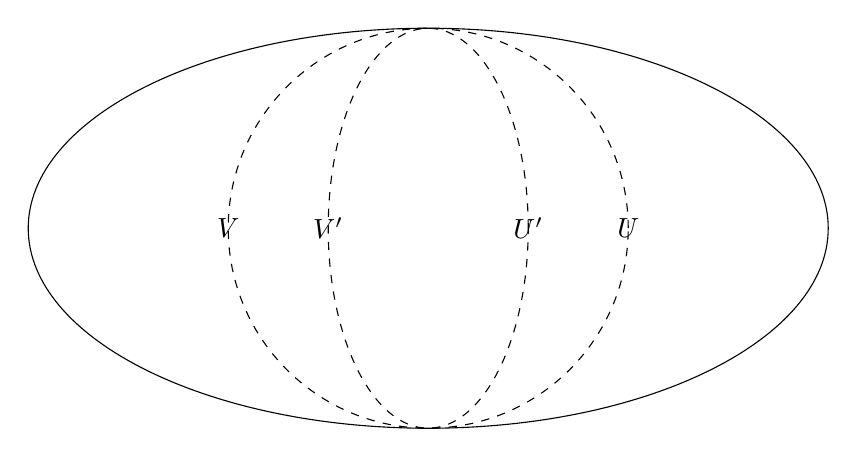
\begin{tikzpicture}
    \draw (0,0) ellipse (2in and 1in);
    \draw [dashed] (0,0) ellipse (1in and 1in);
    \draw [dashed] (0,0) ellipse (0.5in and 1in);
    \node at (1in,0) {\(U\)};
    \node at (0.5in,0) {\(U'\)};
    \node at (-1in,0) {\(V\)};
    \node at (-0.5in,0) {\(V'\)};
  \end{tikzpicture}

  \(X\)
\end{center}

This theorem can be extended to any family of open sets \(\set{U_{\a}:\a\in\l}\) such that:
\[X=\bigcup_{\a\in\l}U_{\a}\]

\newpage

\begin{example}
  \setlength\extrarowheight{2ex}
  \begin{tabular}{|c|c|c|c|c|}
    \hline
    \(SPACE\) & \(T_1\) & \(T_2\) & REGULAR & NORMAL \\
    \hline
    \(R_{\text{std}}\) & \C & \C & \C & \C \\
    \hline
    \(R^n_{\text{std}}\) & \C & \C & \C & \C \\
    \hline
    indiscrete & \X & \X & \X & \X \\
    \hline
    discrete & \C & \C & \C & \C \\
    \hline
    cofinite & \C & \A & \A & \A \\
    \hline
    cocountable & \C & \B & \B & \B \\
    \hline
    \(R_{LL}\) & \C & \C & \C & \C \\
    \hline
    \(R_{+00}\) & \C & \X & \X & \X \\
    \hline
    LOS & \C & \C & \C & \C \\
    \hline
  \end{tabular}

  \bigskip

  \underline{\(R\) and \(\R^n\)}

  Since there is a finite distance between points and closed sets (not containing those points), there is always room
  for enclosing disjoint balls.

  \underline{indiscrete}

  Since the only non-empty set is the entire space, there is no separation.

  \underline{discrete}

  Since all disjoint subsets are both open and closed, they are self-enclosed.

  \underline{cofinite/cocountable}

  First note that all finite sets are closed.  Thus, single points can be viewed as closed sets. So assume \(p\)
  and \(q\) are distinct points in \(X\).  This means that \(X-\set{p}\) and \(X-\set{q}\) are open.  Furthermore,
  \(p\in X-\set{q}\) but \(p\notin X-\set{p}\) and \(q\in X-\set{p}\) but \(q\notin X-\set{q}\).  Thus,
  cofinite/cocountable is \(T_1\).

  Now assume that there exists disjoint \(U,V\in\T\).  This means that \(X-U\) and \(X-V\) are finite/countable and
  since \(U\cap V=\emptyset\) it is the case that \(X-(U\cap V)=(X-U)\cup(X-V)=X\) and hence \(X\) is
  finite/countable.  When \(X\) is finite/countable, all subsets are both open and closed, equivalent to the
  discrete topology, and so cofinite and cocountable are \(T_2\), regular, and normal.  However, if \(X\) is
  infinite/uncountable then open sets will always intersect and so cofinite and countable are neither \(T_2\),
  regular, nor normal.

  \underline{\(\R_{LL}\)}

  Since \(R_{LL}\) is finer than \(\R\), it has the same separation properties.

  \underline{\(\R_{+00}\)}

  Any two points can be \(T_1\) separated using the basis elements; however, if one point or closed set contains
  \(0'\) and the other point or closed set contains \(0''\) then there is always overlap between the two containing
  basis elements.

  \underline{Lexigraphically Ordered Square}

  Use the alternate definitions.  For any point \(p\in X\), there exists some containing open set (strip), and it is
  always possible to use a smaller strip whose closure is contained in the original strip.  For any closed set
  \(A\in X\), \(X-A\) is an enclosing open set, and likewise, a smaller open set with contained closure is possible.
\end{example}

\begin{theorem}
  \(X,Y\) are \(T_2\implies X\times Y\) is \(T_2\).
\end{theorem}

\begin{proof}
  Assume that \(X\) and \(Y\) are \(T_2\) and assume \(p_1,p_2\in X\times Y\) where \(p_1=(x_1,y_1)\) and
  \(p_2=(x_2,y_2)\).  Since \(X\) is \(T_2\), there exists \(U_1,U_2\in\T_X\) such that \(x_1\in U_1\) and
  \(x_2\in U_2\) and \(U_1\cap U_2=\emptyset\).  Likewise, since \(Y\) is \(T_2\), there exists \(V_1,V_2\in\T_Y\)
  such that \(y_1\in V_1\) and \(y_2\in V_2\) and \(V_1\cap V_2=\emptyset\).  So \(p_1\in U_1\times V_1\) and
  \(p_2\in U_2\times V_2\).  Furthermore, \(U_1\times V_1,U_2\times V_2\in\T_{X\times Y}\) and
  \[(U_1\times V_1)\cap(U_2\times V_2)=(U_1\cap U_2)\times(V_1\cap V_2)=\emptyset\]

  Therefore \(X\times Y\) is \(T_2\).
\end{proof}

\begin{lemma}
  Let \(X\) and \(Y\) be topological spaces and let \(A\subset X\) and \(B\subset Y\):
  \[\overline{A\times B}=\bar{A}\times\bar{B}\]
\end{lemma}

\begin{proof}
  Assume that \(p\in\overline{A\times B}\).  This means that for all \(U\in\T_{X\times B}\) such that \(p\in U\):
  \[U\cap(A\times B)\ne\emptyset\]
  Now assume \(U_1\in\T_X\) and \(U_2\in T_Y\) such that \(p\in U_1\times U_2\in\T_{A\times B}\).  Then it must be the
  case that \((U_1\times U_2)\cap(A\times B)=(U_1\cap A)\times(U_2\cap B)\ne\emptyset\).  This is only possible if
  \(U_1\cap A\ne\emptyset\) and \(U_2\cap B\ne\emptyset\).

  Therefore \(p\in\bar{A}\times\bar{B}\).

  Assume that \(p\in\bar{A}\times\bar{B}\).  This means that for all \(U_1\in\T_X\) and \(U_2\in\T_Y\) such that
  \(p\in U_1\times U_2\):
  \[(U_1\cap A)\times(U_2\cap B)\ne\emptyset\]
  Now assume \(U\in\T_{A\times B}\) such that \(p\in U\in\T_{A\times B}\).  Then there exists \(U_1\in\T_X\) and
  \(U_2\in T_Y\) such that \(p\in U_1\times U_2=U\).  So it must be the case that:
  \[U\cap(A\times B)=(U_1\times U_2)\cap(A\times B)=(U_1\cap A)\times(U_2\cap B)\ne\emptyset\]

  Therefore \(p\in\overline{A\times B}\).
\end{proof}

\begin{theorem}
  \(X,Y\) are regular \(\implies X\times Y\) is regular.
\end{theorem}

\begin{proof}
  Assume that \(X\) and \(Y\) are regular and assume \(p\in X\times Y\) and \(U\in\U_p\).  Then there exists
  \(U_1\in\T_X\) and \(U_2\in\T_Y\) such that \(p\in U_1\times U_2\subset U\).  Now, since \(X\) and \(Y\) are
  regular, there exists \(V_1\in\T_X\) and \(V_2\in\T_y\) such that \(p\in V_1\times V_2\),
  \(V_1\subset\overline{V_1}\subset U_1\), and \(V_2\subset\overline{V_2}\subset U_2\).  Furthermore, since
  \(\overline{V_1}\) is closed in \(X\) and \(\overline{V_2}\) is closed in \(Y\),
  \(\overline{V_1}\times\overline{V_2}\) (and hence \(\overline{V_1\times V_2}\)) is closed in \(X\times Y\).
  And so:
  \[p\in V_1\times V_2\subset\overline{V_1\times V_2}=\overline{V_1}\times\overline{V_2}\subset U_1\times U_2\]
  Therefore \(X\times Y\) is regular.
\end{proof}

\end{document}
